

\section{Практическая часть}

\subsection{Методы исследования}

Метод расчета уровня загрязнения СО я позаимствовала у работников ВГУ: Негробов~О.П., Логвиновский~В.Д. и Пантелеева~Н.Ю. В их практикуме мною была найдена специальная формула для расчета того самого загрязнения.

Для оценки загрязнения приземного слоя атмосферного воздуха используется формула (\ref{eq:main}) из \cite{begma}:

\begin{equation}
K_{CO} = (0,5 + 0,01N * K_{\text{Т}}) * K_{\text{А}} * K_{\text{У}} * K_{\text{С}} * K_{\text{В}} * K_{\text{П}},
\label{eq:main}
\end{equation}

\par где $K_{CO}$ – концентрация окиси углерода, мг/м$^3$,
\par 0,5 – фоновое (не транспортное) загрязнение приземного слоя атмосферного воздуха в пределах городской черты Воронежа, мг/м$^3$,
\par N – суммарная интенсивность движения автомобилей на улицах г.~Воронежа (автомобилей/час),
\par $K_{\text{Т}}$ – коэффициент токсичности определенного типа автомобилей по выбросам в атмосферу СО,
\par $K_{\text{А}}$ – коэффициент, учитывающий аэрацию на данном участке дороги (таблица~\ref{t:Ka}),
\par $K_{\text{У}}$ – коэффициент, учитывающий величину уклона дорожного полотна (таблица~\ref{t:Ku}),
\par $K_{\text{С}}$ – коэффициент, учитывающий скорость ветра (таблица~\ref{t:Kc}),
\par $K_{\text{В}}$ – коэффициент, учитывающий влажность воздуха (таблица~\ref{t:Kv}),
\par $K_{\text{П}}$ – коэффициент, учитывающий зависимость концентрации окиси углерода от типа пересечения дорог (таблица~\ref{t:Kp}).


Значение коэффициента токсичности по выбросам в атмосферу СО ($K_{\text{Т}}$) определяется по формуле:
\begin{equation}
K_{\text{Т}} = \sum_{i=1}^{N}P_{i}K_{\text{Т}i},
\label{eq:Kt}
\end{equation}

\par где $P_{i}$ – состав движения (в долях от общего количества транспортного потока),
\par $K_{\text{Т}i}$ – токсичности (по выбросу СО) для каждого вида транспорта.



Для исследования мной были выбраны три остановочных пункта:
\begin{itemize}
\item остановка ''ул. Карла Маркса'';
\item остановка ''Кинотеатр ''Спартак'';
\item остановка ''ТЮЗ''.
\end{itemize}

Ниже на рисунках показаны фрагменты карт с этими остановками.

\begin{figure}[H]%
  \centering
  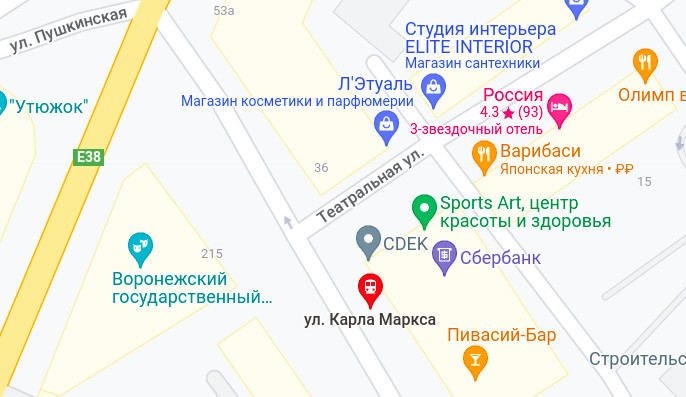
\includegraphics[width=0.8\textwidth]{src/st_k_marks.jpg}
  \caption{Остановка ''ул. Карла Маркса''} \label{p:k_marks}
\end{figure}% scale = 0.3, width=\textwidth

\begin{figure}[H]%
  \centering
  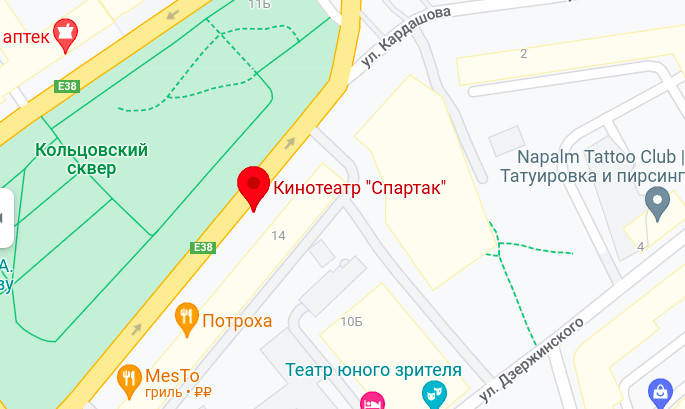
\includegraphics[width=0.8\textwidth]{src/st_spartak.jpg}
  \caption{Остановка ''Кинотеатр ''Спартак''} \label{p:spartak}
\end{figure}% scale = 0.3, width=\textwidth

\begin{figure}[H]%
  \centering
  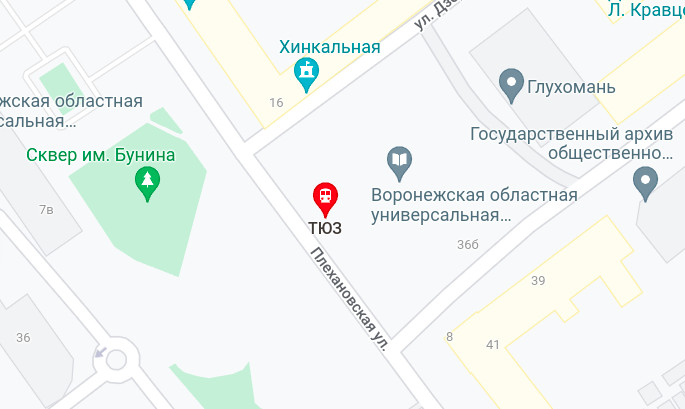
\includegraphics[width=0.8\textwidth]{src/st_tuz.jpg}
  \caption{Остановка ''ТЮЗ''} \label{p:tuz}
\end{figure}% scale = 0.3, width=\textwidth

Мой выбор можно логически обосновать. Все они находятся в шаговой доступности от моего
дома, поэтому измерить уровень загрязнения именно там – жизненная необходимость.

Для всех улиц можно сказать: ''магистральная улица с многоэтажной застройкой с обеих сторон'' (таблица~\ref{t:Ka}).

Для всех улиц можно сказать, что ''продольный уклон 0~\%'' (таблица~\ref{t:Ku}).

Для всех улиц можно сказать, что движение ''регулируемое автоматическими светофорами'' (таблица~\ref{t:Kp}).





Я измерила количество машин, которые проедут мимо каждого пункта за один час.


\subsubsection{Остановка ''ул. Карла Маркса''}



23 ноября 2022~года с 18:00 до 19:00 я проводила подсчеты на остановке ''ул. Карла Маркса'' (рисунок~\ref{p:k_marks}). Результаты приведены в таблице~\ref{t:k_marks}. В этот день был порывистый ветер со скоростью 4~м/сек (таблица~\ref{t:Kc}) и дождь (влажность воздуха 100~\%, таблица~\ref{t:Kv}).

\small
\begin{longtable}{|L{70mm}|C{40mm}|C{30mm}|C{15mm}|}
  \caption{Определение коэффициента токсичности по выбросам в атмосферу СО ($K_{\text{Т}}$) на остановке ''ул. Карла Маркса''} \label{t:k_marks} \\
  \hline
  \rowcolor{Gray}
  \multicolumn{1}{|L{70mm}|}{\centering Тип автотранспортного средства} &
  \multicolumn{1}{C{40mm}|}{\centering Количество автомобилей} &
  \multicolumn{1}{C{30mm}|}{\centering Доля от общего количества транспортного потока ($P_{i}$)} &
  \multicolumn{1}{C{15mm}|}{\centering $K_{\text{Т}i}$} \\\hline
  \endfirsthead
  \caption*{Продолжение таблицы \ref{t:k_marks}} \\
  \hline
  \rowcolor{Gray}
  \multicolumn{1}{|L{70mm}|}{\centering Тип автотранспортного средства} &
  \multicolumn{1}{C{40mm}|}{\centering Количество автомобилей} &
  \multicolumn{1}{C{30mm}|}{\centering Доля от общего количества транспортного потока ($P_{i}$)} &
  \multicolumn{1}{C{15mm}|}{\centering $K_{\text{Т}i}$} \\\hline
  \endhead
   Лёгкий грузовой (в том числе маршрутные такси ''Газель'')             & \directlua{rnd2(t.k_marks.lg.Num)}     & \directlua{rnd3(t.k_marks.lg.Pi)}     & \directlua{rnd2(t.k_marks.lg.Kti)}     \\ \hline
   Средний грузовой (в том числе маршрутные	такси-автобусы ''ПАЗ'')      & \directlua{rnd2(t.k_marks.sg.Num)}     & \directlua{rnd3(t.k_marks.sg.Pi)}     & \directlua{rnd2(t.k_marks.sg.Kti)}     \\ \hline
   Тяжёлый грузовой (дизельные, в том числе маршрутные автобусы)       & \directlua{rnd2(t.k_marks.tg_diz.Num)} & \directlua{rnd3(t.k_marks.tg_diz.Pi)} & \directlua{rnd2(t.k_marks.tg_diz.Kti)} \\ \hline
   Тяжёлый грузовой (с двигателями внутреннего сгорания)               & \directlua{rnd2(t.k_marks.tg_dvs.Num)} & \directlua{rnd3(t.k_marks.tg_dvs.Pi)} & \directlua{rnd2(t.k_marks.tg_dvs.Kti)} \\ \hline
   Легковой                                                            & \directlua{rnd2(t.k_marks.l.Num)}      & \directlua{rnd3(t.k_marks.l.Pi)}      & \directlua{rnd2(t.k_marks.l.Kti)}      \\ \hline
   Всего автомобилей за 1~час                                          & \directlua{rnd2(t.k_marks.summ.Num)}   &                                       & \directlua{rnd2(t.k_marks.summ.Kt)}    \\ \hline
\end{longtable} \normalsize




\subsubsection{Остановка ''Кинотеатр ''Спартак''}

24 ноября 2022~года с 18:00 до 19:00 я проводила подсчеты на остановке ''Кинотеатр ''Спартак'' (рисунок~\ref{p:spartak}). Результаты приведены в таблице~\ref{t:spartak}. В этот день был туман, что означает ветер 0~м/сек (таблица~\ref{t:Kc}) и влажность воздуха 100~\% (таблица~\ref{t:Kv}).

\small
\begin{longtable}{|L{70mm}|C{40mm}|C{30mm}|C{15mm}|}
  \caption{Определение коэффициента токсичности по выбросам в атмосферу СО ($K_{\text{Т}}$) на остановке ''Кинотеатр ''Спартак''} \label{t:spartak} \\
  \hline
  \rowcolor{Gray}
  \multicolumn{1}{|L{70mm}|}{\centering Тип автотранспортного средства} &
  \multicolumn{1}{C{40mm}|}{\centering Количество автомобилей} &
  \multicolumn{1}{C{30mm}|}{\centering Доля от общего количества транспортного потока ($P_{i}$)} &
  \multicolumn{1}{C{15mm}|}{\centering $K_{\text{Т}i}$} \\\hline
  \endfirsthead
  \caption*{Продолжение таблицы \ref{t:spartak}} \\
  \hline
  \rowcolor{Gray}
  \multicolumn{1}{|L{70mm}|}{\centering Тип автотранспортного средства} &
  \multicolumn{1}{C{40mm}|}{\centering Количество автомобилей} &
  \multicolumn{1}{C{30mm}|}{\centering Доля от общего количества транспортного потока ($P_{i}$)} &
  \multicolumn{1}{C{15mm}|}{\centering $K_{\text{Т}i}$} \\\hline
  \endhead
   Лёгкий грузовой (в том числе маршрутные такси ''Газель'')             & \directlua{rnd2(t.k_spartak.lg.Num)}     & \directlua{rnd3(t.k_spartak.lg.Pi)}     & \directlua{rnd2(t.k_spartak.lg.Kti)}     \\ \hline
   Средний грузовой (в том числе маршрутные	такси-автобусы ''ПАЗ'')      & \directlua{rnd2(t.k_spartak.sg.Num)}     & \directlua{rnd3(t.k_spartak.sg.Pi)}     & \directlua{rnd2(t.k_spartak.sg.Kti)}     \\ \hline
   Тяжёлый грузовой (дизельные, в том числе маршрутные автобусы)       & \directlua{rnd2(t.k_spartak.tg_diz.Num)} & \directlua{rnd3(t.k_spartak.tg_diz.Pi)} & \directlua{rnd2(t.k_spartak.tg_diz.Kti)} \\ \hline
   Тяжёлый грузовой (с двигателями внутреннего сгорания)               & \directlua{rnd2(t.k_spartak.tg_dvs.Num)} & \directlua{rnd3(t.k_spartak.tg_dvs.Pi)} & \directlua{rnd2(t.k_spartak.tg_dvs.Kti)} \\ \hline
   Легковой                                                            & \directlua{rnd2(t.k_spartak.l.Num)}      & \directlua{rnd3(t.k_spartak.l.Pi)}      & \directlua{rnd2(t.k_spartak.l.Kti)}      \\ \hline
   Всего автомобилей за 1~час                                          & \directlua{rnd2(t.k_spartak.summ.Num)}   &                                         & \directlua{rnd2(t.k_spartak.summ.Kt)}    \\ \hline
\end{longtable} \normalsize




\subsubsection{Остановка ''ТЮЗ''}

25 ноября 2022~года с 18:00 до 19:00 я проводила подсчеты на остановке ''ТЮЗ'' (рисунок~\ref{p:tuz}). Результаты приведены в таблице~\ref{t:tuz}. В этот день был слабый ветер ( 0~м/сек, таблица~\ref{t:Kc}) и подмораживало (влажность воздуха 40~\%, таблица~\ref{t:Kv}).

\small
\begin{longtable}{|L{70mm}|C{40mm}|C{30mm}|C{15mm}|}
  \caption{Определение коэффициента токсичности по выбросам в атмосферу СО ($K_{\text{Т}}$) на остановке ''ТЮЗ''} \label{t:tuz} \\
  \hline
  \rowcolor{Gray}
  \multicolumn{1}{|L{70mm}|}{\centering Тип автотранспортного средства} &
  \multicolumn{1}{C{40mm}|}{\centering Количество автомобилей} &
  \multicolumn{1}{C{30mm}|}{\centering Доля от общего количества транспортного потока ($P_{i}$)} &
  \multicolumn{1}{C{15mm}|}{\centering $K_{\text{Т}i}$} \\\hline
  \endfirsthead
  \caption*{Продолжение таблицы \ref{t:tuz}} \\
  \hline
  \rowcolor{Gray}
  \multicolumn{1}{|L{70mm}|}{\centering Тип автотранспортного средства} &
  \multicolumn{1}{C{40mm}|}{\centering Количество автомобилей} &
  \multicolumn{1}{C{30mm}|}{\centering Доля от общего количества транспортного потока ($P_{i}$)} &
  \multicolumn{1}{C{15mm}|}{\centering $K_{\text{Т}i}$} \\\hline
  \endhead
   Лёгкий грузовой (в том числе маршрутные такси ''Газель'')             & \directlua{rnd2(t.k_tuz.lg.Num)}     & \directlua{rnd3(t.k_tuz.lg.Pi)}     & \directlua{rnd2(t.k_tuz.lg.Kti)}     \\ \hline
   Средний грузовой (в том числе маршрутные	такси-автобусы ''ПАЗ'')      & \directlua{rnd2(t.k_tuz.sg.Num)}     & \directlua{rnd3(t.k_tuz.sg.Pi)}     & \directlua{rnd2(t.k_tuz.sg.Kti)}     \\ \hline
   Тяжёлый грузовой (дизельные, в том числе маршрутные автобусы)       & \directlua{rnd2(t.k_tuz.tg_diz.Num)} & \directlua{rnd3(t.k_tuz.tg_diz.Pi)} & \directlua{rnd2(t.k_tuz.tg_diz.Kti)} \\ \hline
   Тяжёлый грузовой (с двигателями внутреннего сгорания)               & \directlua{rnd2(t.k_tuz.tg_dvs.Num)} & \directlua{rnd3(t.k_tuz.tg_dvs.Pi)} & \directlua{rnd2(t.k_tuz.tg_dvs.Kti)} \\ \hline
   Легковой                                                            & \directlua{rnd2(t.k_tuz.l.Num)}      & \directlua{rnd3(t.k_tuz.l.Pi)}      & \directlua{rnd2(t.k_tuz.l.Kti)}      \\ \hline
   Всего автомобилей за 1~час                                          & \directlua{rnd2(t.k_tuz.summ.Num)}   &                                     & \directlua{rnd2(t.k_tuz.summ.Kt)}    \\ \hline
\end{longtable} \normalsize





\subsection{Результаты исследования}


После проведения измерений, значения из таблиц~\ref{t:k_marks}-\ref{t:tuz} и из таблиц в приложении~\ref{app:tables} были подставлены в формулу~(\ref{eq:main}). Результаты вычислений были сведены в таблицу~\ref{t:final}.

Еще раз отметим, что предельно допустимая концентрация монооксида углерода в приземном слое атмосферного воздуха в городах Российской Федерации равен \directlua{rnd2(t.PDK)}~мг/м$^3$.

\small
\begin{longtable}{|L{70mm}|C{40mm}|C{40mm}|}
  \caption{Концентрация загрязнения в воздухе на остановочных пунктах} \label{t:final} \\
  \hline
  \rowcolor{Gray}
  \multicolumn{1}{|L{70mm}|}{\centering Название остановочного пункта} &
  \multicolumn{1}{C{40mm}|}{\centering Концентрация загрязнения ($K_{CO}$, мг/м$^3$)} &
  \multicolumn{1}{C{40mm}|}{\centering Превышение ПДК, раз} \\\hline
  \endfirsthead
  \caption*{Продолжение таблицы \ref{t:final}} \\
  \hline
  \rowcolor{Gray}
  \multicolumn{1}{|L{70mm}|}{\centering Название остановочного пункта} &
  \multicolumn{1}{C{40mm}|}{\centering Концентрация загрязнения ($K_{CO}$, мг/м$^3$)} &
  \multicolumn{1}{C{40mm}|}{\centering Превышение ПДК, раз} \\\hline
  \endhead
   Остановка ''ул. Карла Маркса''    & \directlua{rnd2(t.k_marks.summ.Kco)}   & \directlua{rnd1(t.k_marks.summ.mul_PDK)} \\ \hline
   Остановка ''Кинотеатр ''Спартак'' & \directlua{rnd2(t.k_spartak.summ.Kco)} & \directlua{rnd1(t.k_spartak.summ.mul_PDK)}  \\ \hline
   Остановка ''ТЮЗ''                 & \directlua{rnd2(t.k_tuz.summ.Kco)}     & \directlua{rnd1(t.k_tuz.summ.mul_PDK)}  \\ \hline
\end{longtable} \normalsize








\section*{Заключение}

В результате проведенного исследования мы убедились, что наиболее значимыми факторами отрицательного влияния автотранспорта на человека и окружающую среду являются:
\begin{itemize}
\item загрязнение воздуха;
\item загрязнение окружающей среды.
\end{itemize}

Увеличение автомобильного парка порождает и экологические проблемы, связанные с загрязнением воздушного бассейна городов и населенных пунктов. Загрязнение воздуха выхлопами автотранспортных средств представляет серьезную угрозу здоровью населения, способствует снижению качества жизни. Несмотря на проводимые природоохранные мероприятия, экологическая ситуация остается неблагоприятной.

Как видно из результатов исследований в таблице~\ref{t:final}, только ПДК по монооксиду углерода на центральных улицах г.Воронежа превышена в несколько десятков раз. Загрязнение монооксидом углерода все не ограничивается. Преждевременная
потеря здоровья жителями страны, в переводе на экономический язык - ведет к убыткам и издержкам, что замедляет развитие страны на фоне других стран. В переводе на медицинский язык - у людей уменьшается период комфортного существования, что отрицательно сказывается на психическом и психологическом состоянии отдельных людей и общества в целом. Первый шаг к решению проблемы - осознать проблему.

Данный документ создавался с помощью системы \LaTeX. \LaTeX\ - система компьютерного набора, предназначена для создания научных и математических документов высокого типографского качества. Подробнее можно узнать в \cite{Lvovsky} и в \cite{eskdi}. Расчеты проводились с помощью языка Lua \cite{Ierusalimschy}, интегрированного с \LaTeX. Листинг программы с расчетами приведен в приложении~\ref{app:calc}. Такая интеграция позволяет оперативно корректировать расчетные данные в документе, тем самым выводя создание научной и технической документации на новый более высокий уровень.



\begin{thebibliography}{99}
\sectionmark{Список литературы}
  \bibitem{golubev} Голубев, Игорь Родиславович. Окружающая среда и транспорт / И. Р. Голубев, Ю. В. Новиков. - М. : Транспорт, 1987. - 206,[1] с. : ил.; 20 см.

  \bibitem{mihailovsky} Михайловский Е.В. Устройство автомобиля: Учебник для учащихся автотранспортных техникумов - 6-е изд., стереотип. - М.Ж Машиностроение, 1987. - 352 с.: ил.

  \bibitem{begma} Федорова А.И. Практикум по экологии и охране окружающей среды : учеб. пособ. для студ. вузов. /А.И. Федорова., А.Н. Никольская. – М.: Гуманит. изд. центр ''ВЛАДОС'', 2001. – 288 с.

  \bibitem{Lvovsky} С.М.Львовский, Набор и верстка в системе LaTeX. - 5-е изд., переработанное. - М.: МЦНМО, 2014 - 400 с.

  \bibitem{eskdi} Стилевые файлы для TeX Live, позволяющие создавать текстовые документы согласно ЕСКД \url{https://github.com/yrasik/eskdi}.

  \bibitem{Ierusalimschy} Иерузалимский Р. - Программирование на языке Lua. 3-е издание / пер. с англ. А.В.Боресков - М.: ДМК Пресс, 2016. -382 с.: ил.

\end{thebibliography}





\appendix % Приложения. Можно разместить перед списком литературы - тогда список литературы оформится как приложение


\section[Коэффициенты для расчета уровня загрязнения СО]{Справочное} \label{app:tables}


\small
\begin{longtable}{|L{100mm}|C{50mm}|}
  \caption{Зависимость аэрации конкретного участка автодороги от её типа и типа прилегающих к ней застроек} \label{t:Ka} \\
  \hline
  \rowcolor{Gray}
  \multicolumn{1}{|L{100mm}|}{\centering Тип участка дороги по степени аэрации} &
  \multicolumn{1}{C{50mm}|}{\centering Коэффициент аэрации ($K_{\text{А}}$)} \\\hline
  \endfirsthead
  \caption*{Продолжение таблицы \ref{t:Ka}} \\
  \hline
  \rowcolor{Gray}
  \multicolumn{1}{|L{100mm}|}{\centering Тип участка дороги по степени аэрации} &
  \multicolumn{1}{C{50mm}|}{\centering Коэффициент аэрации ($K_{\text{А}}$)} \\\hline
  \endhead
   Транспортные тоннели      & \directlua{rnd2(t.Ka.tt)} \\ \hline
   Транспортные галереи      & \directlua{rnd2(t.Ka.tg)} \\ \hline
   Магистральные улицы и дороги с многоэтажной застройкой с обеих сторон                              & \directlua{rnd2(t.Ka.mu)} \\ \hline
   Жилые улицы с одноэтажной застройкой, улицы и дороги в выемке                                      & \directlua{rnd2(t.Ka.ghu)} \\ \hline
   Городские улицы и дороги с односторонней застройкой, набережные эстакады, виадуки, высокие насыпи  & \directlua{rnd2(t.Ka.gu)} \\ \hline
\end{longtable} \normalsize


\small
\begin{longtable}{|C{100mm}|C{50mm}|}
  \caption{Зависимость загрязнения воздуха окисью углерода от величины уклона дорожного полотна} \label{t:Ku} \\
  \hline
  \rowcolor{Gray}
  \multicolumn{1}{|C{100mm}|}{\centering Продольный уклон (в~\%)} &
  \multicolumn{1}{C{50mm}|}{\centering Коэффициент уклона дорожного полотна ($K_{\text{У}}$)} \\\hline
  \endfirsthead
  \caption*{Продолжение таблицы \ref{t:Ku}} \\
  \hline
  \rowcolor{Gray}
  \multicolumn{1}{|C{100mm}|}{\centering Продольный уклон (в~\%)} &
  \multicolumn{1}{C{50mm}|}{\centering Коэффициент уклона дорожного полотна ($K_{\text{У}}$)} \\\hline
  \endhead
    0  & \directlua{rnd2(t.Ku.g_0)} \\ \hline
    2  & \directlua{rnd2(t.Ku.g_2)} \\ \hline
    4  & \directlua{rnd2(t.Ku.g_4)} \\ \hline
    6  & \directlua{rnd2(t.Ku.g_6)} \\ \hline
    8  & \directlua{rnd2(t.Ku.g_8)} \\ \hline
\end{longtable} \normalsize


\small
\begin{longtable}{|L{100mm}|C{50mm}|}
  \caption{Зависимость изменения в воздухе концентрации окиси углерода от типа пересечения дорог} \label{t:Kp} \\
  \hline
  \rowcolor{Gray}
  \multicolumn{1}{|L{100mm}|}{\centering Тип движения и пересечения дорог} &
  \multicolumn{1}{C{50mm}|}{\centering Коэффициент концентрации окиси углерода ($K_{\text{П}}$)} \\\hline
  \endfirsthead
  \caption*{Продолжение таблицы \ref{t:Kp}} \\
  \hline
  \rowcolor{Gray}
  \multicolumn{1}{|L{100mm}|}{\centering Тип движения и пересечения дорог} &
  \multicolumn{1}{C{50mm}|}{\centering Коэффициент концентрации окиси углерода ($K_{\text{П}}$)} \\\hline
  \endhead
    Регулируемое:                &                                        \\
    \hspace{1cm} светофорами автоматическими  & \directlua{rnd2(t.Kp.svet_auto)} \\
    \hspace{1cm} светофорами управляемыми     & \directlua{rnd2(t.Kp.svet_direct)} \\ \hline
    Нерегулируемое:              &                                        \\
    \hspace{1cm} обычный перекрёсток     & \directlua{rnd2(t.Kp.crossroads_simple)} \\ 
    \hspace{1cm} с круговым движением     & \directlua{rnd2(t.Kp.crossroads_round)} \\
    \hspace{1cm} с обязательной остановкой     & \directlua{rnd2(t.Kp.crossroads_stop)} \\ \hline
\end{longtable} \normalsize




\small
\begin{longtable}{|C{100mm}|C{50mm}|}
  \caption{Зависимость изменения в воздухе концентрации окиси углерода от скорости ветра} \label{t:Kc} \\
  \hline
  \rowcolor{Gray}
  \multicolumn{1}{|C{100mm}|}{\centering Скорость ветра, м/сек.} &
  \multicolumn{1}{C{50mm}|}{\centering Коэффициент концентрации окиси углерода от скорости ветра ($K_{\text{С}}$)} \\\hline
  \endfirsthead
  \caption*{Продолжение таблицы~\ref{t:Kc}} \\
  \hline
  \rowcolor{Gray}
  \multicolumn{1}{|C{100mm}|}{\centering Скорость ветра, м/сек.} &
  \multicolumn{1}{C{50mm}|}{\centering Коэффициент концентрации окиси углерода от скорости ветра ($K_{\text{С}}$)} \\\hline
  \endhead
    1  & \directlua{rnd2(t.Kc.v_1)} \\ \hline
    2  & \directlua{rnd2(t.Kc.v_2)} \\ \hline
    3  & \directlua{rnd2(t.Kc.v_3)} \\ \hline
    4  & \directlua{rnd2(t.Kc.v_4)} \\ \hline
    5  & \directlua{rnd2(t.Kc.v_5)} \\ \hline
    6  & \directlua{rnd2(t.Kc.v_6)} \\ \hline
\end{longtable} \normalsize


\small
\begin{longtable}{|C{100mm}|C{50mm}|}
  \caption{Зависимость изменения в воздухе концентрации окиси углерода от относительной влажности воздуха} \label{t:Kv} \\
  \hline
  \rowcolor{Gray}
  \multicolumn{1}{|C{100mm}|}{\centering Относительная влажность воздуха (в~\%)} &
  \multicolumn{1}{C{50mm}|}{\centering Коэффициент концентрации окиси углерода от относительной влажности ($K_{\text{В}}$)} \\\hline
  \endfirsthead
  \caption*{Продолжение таблицы \ref{t:Kv}} \\
  \hline
  \rowcolor{Gray}
  \multicolumn{1}{|C{100mm}|}{\centering Относительная влажность воздуха (в~\%)} &
  \multicolumn{1}{C{50mm}|}{\centering Коэффициент концентрации окиси углерода от относительной влажности ($K_{\text{В}}$)} \\\hline
  \endhead
    100 & \directlua{rnd2(t.Kv.v_100)} \\ \hline
    90  & \directlua{rnd2(t.Kv.v_90)} \\ \hline
    80  & \directlua{rnd2(t.Kv.v_80)} \\ \hline
    70  & \directlua{rnd2(t.Kv.v_70)} \\ \hline
    60  & \directlua{rnd2(t.Kv.v_60)} \\ \hline
    50  & \directlua{rnd2(t.Kv.v_50)} \\ \hline
    40  & \directlua{rnd2(t.Kv.v_40)} \\ \hline
\end{longtable} \normalsize




\section[Листинг программы расчета загрязнения приземного слоя атмосферного воздука CO]{Рекомендуемое} \label{app:calc}

\inputminted[fontsize=\footnotesize, breaklines, numbersep=0mm, xleftmargin=0mm, frame=single]{lua}{./calc_pollution.lua}



%\section[График функции]{Рекомендуемое} \label{app:graph}

%\begin{figure}[H]%
%  \centering
%  \includegraphics[width=1.0\textwidth]{./graph/graph.pdf}
%  \caption{График функции} \label{pic:graph}
%\end{figure}% scale = 0.3, width=\textwidth

